%%%%%%%%%%%%%%%%%%%%%%%%%%%%%%%%%%%%%%%%%%%%%%%%%%%%%%%%%%%%%%%%%%%%%%%%%%%%%%%
%                                Basic Packages                               %
%%%%%%%%%%%%%%%%%%%%%%%%%%%%%%%%%%%%%%%%%%%%%%%%%%%%%%%%%%%%%%%%%%%%%%%%%%%%%%%

% Gives us multiple colors.
\usepackage[usenames,dvipsnames,pdftex]{xcolor}
% Lets us style link colors.
\usepackage{hyperref}
% Lets us import images and graphics.
\usepackage{graphicx}
% Lets us use figures in floating environments.
\usepackage{float}
% Lets us create multiple columns.
\usepackage{multicol}
% Gives us better math syntax.
\usepackage{amsmath,amsfonts,mathtools,amsthm,amssymb}
% Lets us strikethrough text.
\usepackage{cancel}
% Lets us edit the caption of a figure.
\usepackage{caption}
% Lets us import pdf directly in our tex code.
\usepackage{pdfpages}
% Lets us do algorithm stuff.
\usepackage[ruled,vlined,linesnumbered]{algorithm2e}
% Use a smiley face for our qed symbol.
\usepackage{tikzsymbols}
\renewcommand\qedsymbol{$\Laughey$}
\usepackage{bm}
\renewcommand{\vec}[1]{\boldsymbol{\mathbf{#1}}}
% use Package mathtools
\usepackage{mathtools}
\usepackage{leftindex}
\def\class{article}


%%%%%%%%%%%%%%%%%%%%%%%%%%%%%%%%%%%%%%%%%%%%%%%%%%%%%%%%%%%%%%%%%%%%%%%%%%%%%%%
%                                Basic Settings                               %
%%%%%%%%%%%%%%%%%%%%%%%%%%%%%%%%%%%%%%%%%%%%%%%%%%%%%%%%%%%%%%%%%%%%%%%%%%%%%%%

%%%%%%%%%%%%%
%  Symbols  %
%%%%%%%%%%%%%

\let\implies\Rightarrow
\let\impliedby\Leftarrow
\let\iff\Leftrightarrow
\let\epsilon\varepsilon

%%%%%%%%%%%%
%  Tables  %
%%%%%%%%%%%%

\setlength{\tabcolsep}{5pt}
\renewcommand\arraystretch{1.5}

%%%%%%%%%%%%%%
%  SI Unitx  %
%%%%%%%%%%%%%%

\usepackage{siunitx}
\sisetup{locale = FR}

%%%%%%%%%%
%  TikZ  %
%%%%%%%%%%

\usepackage[framemethod=TikZ]{mdframed}
\usepackage{tikz}
\usepackage{tikz-cd}
\usepackage{tikzsymbols}

\usetikzlibrary{intersections, angles, quotes, calc, positioning}
\usetikzlibrary{arrows.meta}

\tikzset{
  force/.style={thick, {Circle[length=2pt]}-stealth, shorten <=-1pt}
}

%%%%%%%%%%%%%%%
%  PGF Plots  %
%%%%%%%%%%%%%%%

\usepackage{pgfplots}
\pgfplotsset{compat=1.13}

%%%%%%%%%%%%%%%%%%%%%%%
%  Center Title Page  %
%%%%%%%%%%%%%%%%%%%%%%%

\usepackage{titling}
\renewcommand\maketitlehooka{\null\mbox{}\vfill}
\renewcommand\maketitlehookd{\vfill\null}

%%%%%%%%%%%%%%%%%%%%%%%%%%%%%%%%%%%%%%%%%%%%%%%%%%%%%%%
%  Create a grey background in the middle of the PDF  %
%%%%%%%%%%%%%%%%%%%%%%%%%%%%%%%%%%%%%%%%%%%%%%%%%%%%%%%

\usepackage{eso-pic}
\newcommand\definegraybackground{
  \definecolor{reallylightgray}{HTML}{FAFAFA}
  \AddToShipoutPicture{
    \ifthenelse{\isodd{\thepage}}{
      \AtPageLowerLeft{
        \put(\LenToUnit{\dimexpr\paperwidth-222pt},0){
          \color{reallylightgray}\rule{222pt}{297mm}
        }
      }
    }
    {
      \AtPageLowerLeft{
        \color{reallylightgray}\rule{222pt}{297mm}
      }
    }
  }
}

%%%%%%%%%%%%%%%%%%%%%%%%
%  Modify Links Color  %
%%%%%%%%%%%%%%%%%%%%%%%%

\hypersetup{
  % Enable highlighting links.
  colorlinks,
  % Change the color of links to blue.
  linkcolor=blue,
  % Change the color of citations to black.
  citecolor={black},
  % Change the color of url's to blue with some black.
  urlcolor={blue!80!black}
}

%%%%%%%%%%%%%%%%%%
% Fix WrapFigure %
%%%%%%%%%%%%%%%%%%

\newcommand{\wrapfill}{\par\ifnum\value{WF@wrappedlines}>0
    \parskip=0pt
    \addtocounter{WF@wrappedlines}{-1}%
    \null\vspace{\arabic{WF@wrappedlines}\baselineskip}%
    \WFclear
\fi}

%%%%%%%%%%%%%%%%%
% Multi Columns %
%%%%%%%%%%%%%%%%%

\let\multicolmulticols\multicols
\let\endmulticolmulticols\endmulticols

\RenewDocumentEnvironment{multicols}{mO{}}
{%
  \ifnum#1=1
    #2%
  \else % More than 1 column
    \multicolmulticols{#1}[#2]
  \fi
}
{%
  \ifnum#1=1
\else % More than 1 column
  \endmulticolmulticols
\fi
}

\newlength{\thickarrayrulewidth}
\setlength{\thickarrayrulewidth}{5\arrayrulewidth}


%%%%%%%%%%%%%%%%%%%%%%%%%%%%%%%%%%%%%%%%%%%%%%%%%%%%%%%%%%%%%%%%%%%%%%%%%%%%%%%
%                           School Specific Commands                          %
%%%%%%%%%%%%%%%%%%%%%%%%%%%%%%%%%%%%%%%%%%%%%%%%%%%%%%%%%%%%%%%%%%%%%%%%%%%%%%%

%%%%%%%%%%%%%%%%%%%%%%%%%%%
%  Initiate New Counters  %
%%%%%%%%%%%%%%%%%%%%%%%%%%%

\newcounter{lecturecounter}

%%%%%%%%%%%%%%%%%%%%%%%%%%
%  Helpful New Commands  %
%%%%%%%%%%%%%%%%%%%%%%%%%%

\makeatletter

\newcommand\resetcounters{
  % Reset the counters for subsection, subsubsection and the definition
  % all the custom environments.
  \setcounter{subsection}{0}
  \setcounter{subsubsection}{0}
  \setcounter{paragraph}{0}
  \setcounter{subparagraph}{0}
  \setcounter{theorem}{0}
  \setcounter{claim}{0}
  \setcounter{corollary}{0}
  \setcounter{lemma}{0}
  \setcounter{exercise}{0}

  \@ifclasswith\class{nocolor}{
    \setcounter{definition}{0}
  }{}
}

%%%%%%%%%%%%%%%%%%%%%
%  Lecture Command  %
%%%%%%%%%%%%%%%%%%%%%

\usepackage{xifthen}

% EXAMPLE:
% 1. \lesson{Oct 17 2022 Mon (08:46:48)}{Lecture Title}
% 2. \lesson[4]{Oct 17 2022 Mon (08:46:48)}{Lecture Title}
% 3. \lesson{Oct 17 2022 Mon (08:46:48)}{}
% 4. \lesson[4]{Oct 17 2022 Mon (08:46:48)}{}
% Parameters:
% 1. (Optional) Lesson number.
% 2. Time and date of lecture.
% 3. Lecture Title.
\def\@lesson{}
\newcommand\lesson[3][\arabic{lecturecounter}]{
  % Add 1 to the lecture counter.
  \addtocounter{lecturecounter}{1}

  % Set the section number to the lecture counter.
  \setcounter{section}{#1}
  \renewcommand\thesubsection{#1.\arabic{subsection}}

  % Reset the counters.
  \resetcounters

  % Check if user passed the lecture title or not.
  \ifthenelse{\isempty{#3}}{
    \def\@lesson{Lecture \arabic{lecturecounter}}
  }{
    \def\@lesson{Lecture \arabic{lecturecounter}: #3}
  }

  % Display the information like the following:
  %                                                  Oct 17 2022 Mon (08:49:10)
  % ---------------------------------------------------------------------------
  % Lecture 1: Lecture Title
  \hfill\small{#2}
  \hrule
  \vspace*{-0.3cm}
  \section*{\@lesson}
  \addcontentsline{toc}{section}{\@lesson}
}


%%%%%%%%%%%%%%%%%%%%
%  Import Figures  %
%%%%%%%%%%%%%%%%%%%%

\usepackage{import}
\pdfminorversion=7

% EXAMPLE:
% 1. \incfig{limit-graph}
% 2. \incfig[0.4]{limit-graph}
% Parameters:
% 1. The figure name. It should be located in figures/NAME.tex_pdf.
% 2. (Optional) The width of the figure. Example: 0.5, 0.35.
\newcommand\incfig[2][1]{%
  \def\svgwidth{#1\columnwidth}
  \import{./figures/}{#2.pdf_tex}
}

\begingroup\expandafter\expandafter\expandafter\endgroup
\expandafter\ifx\csname pdfsuppresswarningpagegroup\endcsname\relax
\else
  \pdfsuppresswarningpagegroup=1\relax
\fi

%%%%%%%%%%%%%%%%%
% Fancy Headers %
%%%%%%%%%%%%%%%%%

\usepackage{fancyhdr}

% Force a new page.
\newcommand\forcenewpage{\clearpage\mbox{~}\clearpage\newpage}

% This command makes it easier to manage my headers and footers.
\newcommand\createintro{
  % Use roman page numbers (e.g. i, v, vi, x, ...)
  \pagenumbering{roman}

  % Display the page style.
  \maketitle
  % Make the title pagestyle empty, meaning no fancy headers and footers.
  \thispagestyle{empty}
  % Create a newpage.
  \newpage

  % Input the intro.tex page if it exists.
  \IfFileExists{intro.tex}{ % If the intro.tex file exists.
    % Input the intro.tex file.
    \section{Kinematics: Describing the Motions of Spacecraft}
\subsection{Introduction to Kinematics}

\subsubsection{Particle Kinematics and Vector Frames}
\label{sub_sec:Particle Kinematics and Vector Frames}
Something with direction and magnitude.

\[
	\begin{aligned}
		\bm{r} & = x \bm{{\hat{e}_{1}}} + y \bm{{\hat{e}_{2}}} + z \bm{{\hat{e}_{3}}} \\
		       & = r \bm{{\hat{e}_{r}}}                                               \\
		       & = \prescript{\mathcal{E}}{}{
			\begin{bmatrix}
				x \\
				y \\
				z
			\end{bmatrix}
		}                                                                             \\
	\end{aligned}
\]

\begin{example}
	Let the frame \(\mathcal{E} \) be defined as: \(\mathcal{E} \colon \{ \hat{e} _1, \hat{e} _2, \hat{e} _3\} \), with the vector, \(\bm{q}  = 3 \bm{{\hat{e}_{1}}} + 2\bm{{\hat{e}_{3}}} \).\\
	Thus, the vector \(\bm{q} \) can be written in matrix form as:
	\[
		\bm{q}  = \prescript{\mathcal{E}}{}{
			\begin{bmatrix}
				3 \\
				0 \\
				2
			\end{bmatrix}
		}
	\]
\end{example}
\subsubsection*{Coordinate Frames}
\label{subsub_sec:Coordinate Frames}
Let a coordinate frame \(\mathcal{B} \) be defined through 3 unit orthogonal vectors, \( \{ \bm{{\hat{b}_{1}}} , \bm{{\hat{b}_{2}}} , \bm{{\hat{b}_{3}}}  \} \). Let the origin of the frame be given by \( \mathcal{O} _\mathcal{B} \). Then the frame is defined as:
\[
	\mathcal{B} \colon \{ \mathcal{O} _\mathcal{B} , \bm{{\hat{b}_{1}}} , \bm{{\hat{b}_{2}}} , \bm{{\hat{b}_{3}}}  \}
\]
Often the frame origin is ignored, and the shorthand notation is used to define the frame as:
\[
	\mathcal{B} \colon \{ \bm{{\hat{b}_{1}}} , \bm{{\hat{b}_{2}}} , \bm{{\hat{b}_{3}}}  \}
\]

\subsubsection*{Angular Velocity}
The angular velocity vector of a rigid body is often defined as:
\[
	\begin{aligned}
		\bm{\omega }                       & = \omega _1 \bm{{\hat{b}_{1}}} + \omega _2 \bm{{\hat{b}_{2}}} + \omega _3 \bm{{\hat{b}_{3}}} \\
		\prescript{\mathcal{B}}{}{\omega } & = \prescript{\mathcal{B}}{}{
			\begin{bmatrix}
				\omega _1 \\
				\omega _2 \\
				\omega _3
			\end{bmatrix}
		}
	\end{aligned}
\]
where, \(\omega _1, \omega _2, \omega _3 \) are the instantaneous angular velocities about the \(\bm{{\hat{b}_{1}}} , \bm{{\hat{b}_{2}}} , \bm{{\hat{b}_{3}}} \) axes respectively. The angular velocity frame components is shown in \autoref{fig:angularVelocityFrameComponents}.
\begin{figure}[H]
	\centering
	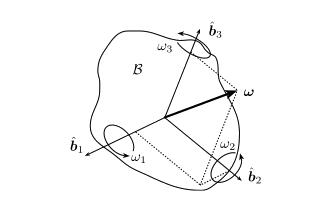
\includegraphics[width=0.5\linewidth]{figures/dynamics/angular_vel.png}
	\caption{Angular velocity body frame components}
	\label{fig:angularVelocityFrameComponents}
\end{figure}

\subsubsection*{Rotation about a Fixed Axis}
Let a body \(\mathcal{B} \) rotate about the axis \(AB\) as shown in \autoref{fig:rotationAboutFixedAxis}. Let the origin \(\mathcal{O} \) of the coordinate system \(\mathcal{B} \) located on the axis of rotation. Let \(P\) be a body fixed point located relative to \(O\) by the vector \(\bm{r} \). Thus, if the vector \(\bm{r} \) is defined in the \(\mathcal{B} \) frame, then the following can be said, from the geometery of the problem:
\[
	\begin{aligned}
		\vert \bm{\dot{r} }  \vert & = (r \sin \theta)  \omega    \\
		\bm{\dot{r} }              & = \bm{\omega } \times \bm{r} \\
	\end{aligned}
\]
\begin{figure}[H]
	\centering
	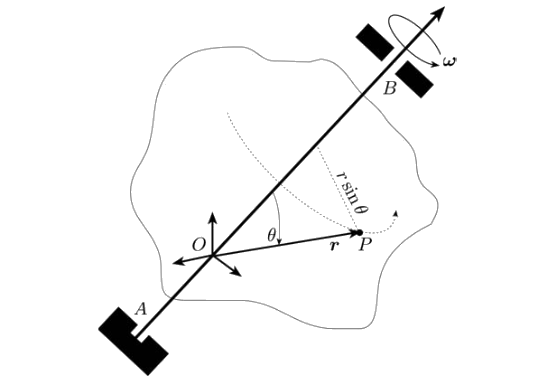
\includegraphics[width=0.5\linewidth]{figures/dynamics/rotationAboutFixedAxis.png}
	\caption{Rotation about a fixed axis}
	\label{fig:rotationAboutFixedAxis}
\end{figure}

\subsubsection{Vector Differentiation and Transport Theorem}
% Vector Differention subsection
\label{subsub_sec:Vector Differentiation}

Let \(\mathcal{N} \) be an inertially fixed frame denoted by the traid, \( \{\bm{{\hat{n}_{1}}}, \bm{{\hat{n}_{2}}}, \bm{{\hat{n}_{3}}}\} \). Let \(\mathcal{B} \) be a another frame denoted by the traid, \( \{\bm{{\hat{b}_{1}}}, \bm{{\hat{b}_{2}}}, \bm{{\hat{b}_{3}}} \}\). For simplicity, the let the origin of the two frames coincide.

Let \(\bm{r}\) be a vector in \(\mathcal{B} \) frame,
\[
	\bm{r} = r_{1}\bm{{\hat{b}_{1}}} + r_{2}\bm{{\hat{b}_{2}}} + r_{3}\bm{{\hat{b}_{3}}}
\]

Let the angular velocity vector \(\omega_{\mathcal{B} / \mathcal{N} }\) define the angular velocity of the \(\mathcal{B} \) frame with respect to the \(\mathcal{N} \) frame. The angular velocity vector is defined usually in the \(\mathcal{B} \) frame as,
\[
	\omega_{\mathcal{B} / \mathcal{N} } = \omega_{1}\bm{{\hat{b}_{1}}} + \omega_{2}\bm{{\hat{b}_{2}}} + \omega_{3}\bm{{\hat{b}_{3}}}
\]
To denote that a derivative of a vector \(\bm{r} \) as seen by the \(\mathcal{B} \) frame, we use the notation,
\[
	\prescript{\mathcal{B}}{}{\frac{d\bm{x}}{{dt}}}{}
\]
The derivative of the vector \(\bm{r} \) as seen by the \(\mathcal{B} \) frame is given by,
\[
	\begin{aligned}
		\prescript{\mathcal{B}}{}{\frac{d\bm{r}}{{dt}}}{dt} & = \prescript{\mathcal{B}}{}{\frac{d}{dt}\left(
			r_{1}\bm{{\hat{b}_{1}}} + r_{2}\bm{{\hat{b}_{2}}} + r_{3}\bm{{\hat{b}_{3}}}
			\right)}                                                                                                                                           \\
		                                                    & =\dot{r}_1 \bm{{\hat{b}_{1}}}  + \dot{r}_2 \bm{{\hat{b}_{2}}} + \dot{r}_3 \bm{{\hat{b}_{3}}}
	\end{aligned}
\]
Since the derivative of the unit vectors \(\bm{{\hat{b}_{i}}}\) wrt the frame \(\mathcal{B} \) is 0.

Using chain rule of differentiation, we can write,
% \[
% 	\prescript{\mathcal{N}}{}{\frac{d}{dt} \bm{r} } =\dot{r}_1 \bm{{\hat{b}_{1}}}  + \dot{r}_2 \bm{{\hat{b}_{2}}} + \dot{r}_3 \bm{{\hat{b}_{3}}} + r_1 \prescript{\mathcal{N}}{}{\frac{d}{dt}\bm{b_1}} + r_2 \prescript{\mathcal{N}}{}{\frac{d}{dt}\bm{b_2} + r_3 \prescript{\mathcal{N}}{}{\frac{d}{dt}\bm{b_3}}}{}{}
% \]
\[
    \leftindex[I]^{\mathcal{N}} {\frac{d}{dt}}
\]
And,
\[
	\prescript{\mathcal{N}}{}{\frac{d}{dt}\bm{{\hat{b}_{i}}} } =  \bm{\omega_{\mathcal{B} / \mathcal{N} }} \times \bm{{\hat{b}_{i}}}
\]
Thus, combining the above two equations, we get,
\[
	\prescript{\mathcal{N}}{}{\frac{d}{dt} \bm{r} } = \prescript{\mathcal{B}}{}{\frac{d\bm{r}}{{dt}}}{} + \bm{\omega_{\mathcal{B} / \mathcal{N} }} \times \bm{r}
\]
\begin{theorem}[Transport Theorem]
	Let \(\mathcal{N} \) and \(\mathcal{B} \) be two frames with a relative angular velocity \(\bm{\omega_{\mathcal{B} / \mathcal{N} }} \). Let \(\bm{r} \) be a generic vector. Then the derivative of the vector \(\bm{r} \) as seen by the \(\mathcal{N} \) frame can be related to the derivative of the vector \(\bm{r} \) as seen by the \(\mathcal{B} \) frame as,
	\[
		\prescript{\mathcal{N}}{}{\frac{d}{dt} \bm{r} } = \prescript{\mathcal{B}}{}{\frac{d\bm{r}}{{dt}}}{} + \bm{\omega_{\mathcal{B} / \mathcal{N} }} \times \bm{r}
	\]
\end{theorem}

\begin{note}
	When writing compact notations, the following will hold,
	\[
		\prescript{\mathcal{N}}{}{\frac{d}{dt}\bm{x} } \equiv \bm{\dot{x} }
	\]
\end{note}

\begin{example}
	\label{ex:planar_transport_thm}
	Find the inertial velocity of the point \(S\) shown in \autoref{fig:planar_transport_thm_ex}
	\begin{figure}[H]
		\centering
		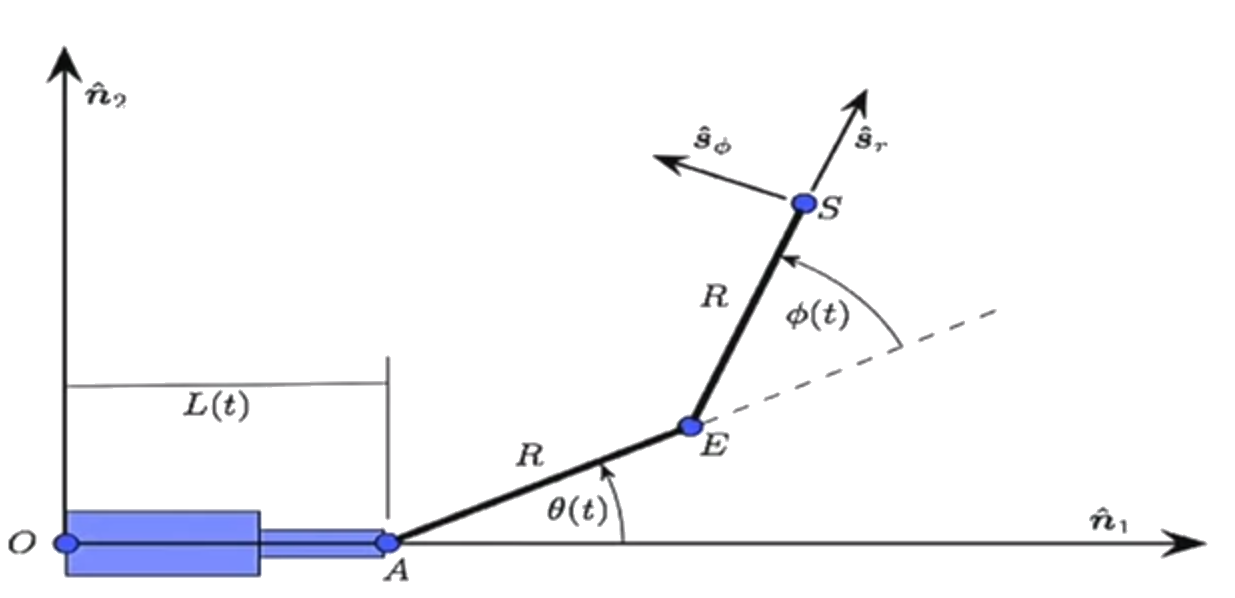
\includegraphics[width=\linewidth]{figures/dynamics/planar_transport_thm_ex.png}
		\caption{Figure for \autoref{ex:planar_transport_thm}}
		\label{fig:planar_transport_thm_ex}
	\end{figure}
	Assigning the frames we have,
	\[
		\begin{aligned}
			\mathcal{N} & \colon  \{ \bm{{\hat{n}_{1}}} , \bm{{\hat{n}_{2}}} , \bm{{\hat{n}_{3}}}  \}       \\
			\mathcal{E} & \colon  \{ \bm{{\hat{e}_{r}}} , \bm{{\hat{e}_{\theta }}} , \bm{{\hat{n}_{3}}}  \} \\
			\mathcal{S} & \colon  \{ \bm{{\hat{s}_{r}}} , \bm{{\hat{s}_{\phi }}} , \bm{{\hat{n}_{3}}}  \}   \\
		\end{aligned}
	\]
	And the angular velocities of the frames relative to each other can be expressed as:
	\[
		\begin{aligned}
			\bm{\omega _{\mathcal{E} / \mathcal{N} }} & = \dot{ \theta} \bm{{\hat{n}_{3}}}                                                    \\
			\bm{\omega _{\mathcal{S} / \mathcal{E} }} & = \dot{ \phi} \bm{{\hat{n}_{3}}}                                                      \\
			\bm{\omega _{\mathcal{S} / \mathcal{N} }} & = \bm{\omega _{\mathcal{E} / \mathcal{N} }}+\bm{\omega _{\mathcal{S} / \mathcal{E} }} \\
			                                          & = (\dot{ \theta} + \dot{ \phi}) \bm{{\hat{n}_{3}}}                                    \\
		\end{aligned}
	\]
	Thus,
	\[
		\begin{aligned}
			\bm{\dot{r} } & = L \bm{{\hat{n}_{1}}} + R \bm{{\hat{e}_{r}}} + R \bm{{\hat{s}_{r}}}                                                                                                                                                                              \\
			              & = \prescript{\mathcal{N}}{}{\frac{d}{dt}\bm{r}} = \prescript{\mathcal{N}}{}{\frac{d}{dt}} L \bm{{\hat{n}_{1}}} + \prescript{\mathcal{E}}{}{\frac{d}{dt}}R \bm{{\hat{e}_{r}}} + \bm{\omega _{\mathcal{E} / \mathcal{N} }} (R \bm{{\hat{e}_{r}}}) +
			\prescript{\mathcal{S}}{}{\frac{d}{dt}}R \bm{{\hat{s}_{r}}} + \bm{\omega _{\mathcal{S} / \mathcal{N} }} (R \bm{{\hat{s}_{r}}})                                                                                                                                    \\
			              & = \dot{L} \bm{{\hat{n}_{1}}} + (\dot{\theta }\bm{{\hat{n}_{3}}} ) \times R \bm{{\hat{e}_{r}}} + \left(
			\dot{\theta}+ \dot{\phi }\right)  \bm{{\hat{n}_{3}}} \times R \bm{{\hat{e}_{r}}}
			\\
			              & = \dot{L}\bm{{\hat{n}_{1}}} + R \dot{\theta } \bm{{\hat{e}_{\theta }}} + R \left(
			\dot{\theta } + \dot{\phi }
			\right)  \bm{{\hat{s}_{\phi }}}
		\end{aligned}
	\]
\end{example}

\begin{example}
	\label{ex:3dtransport_thm}
	Find the inertial velocity of the point \(P\) shown in \autoref{fig:3dtansport_thm_ex}
	\begin{figure}[H]
		\centering
		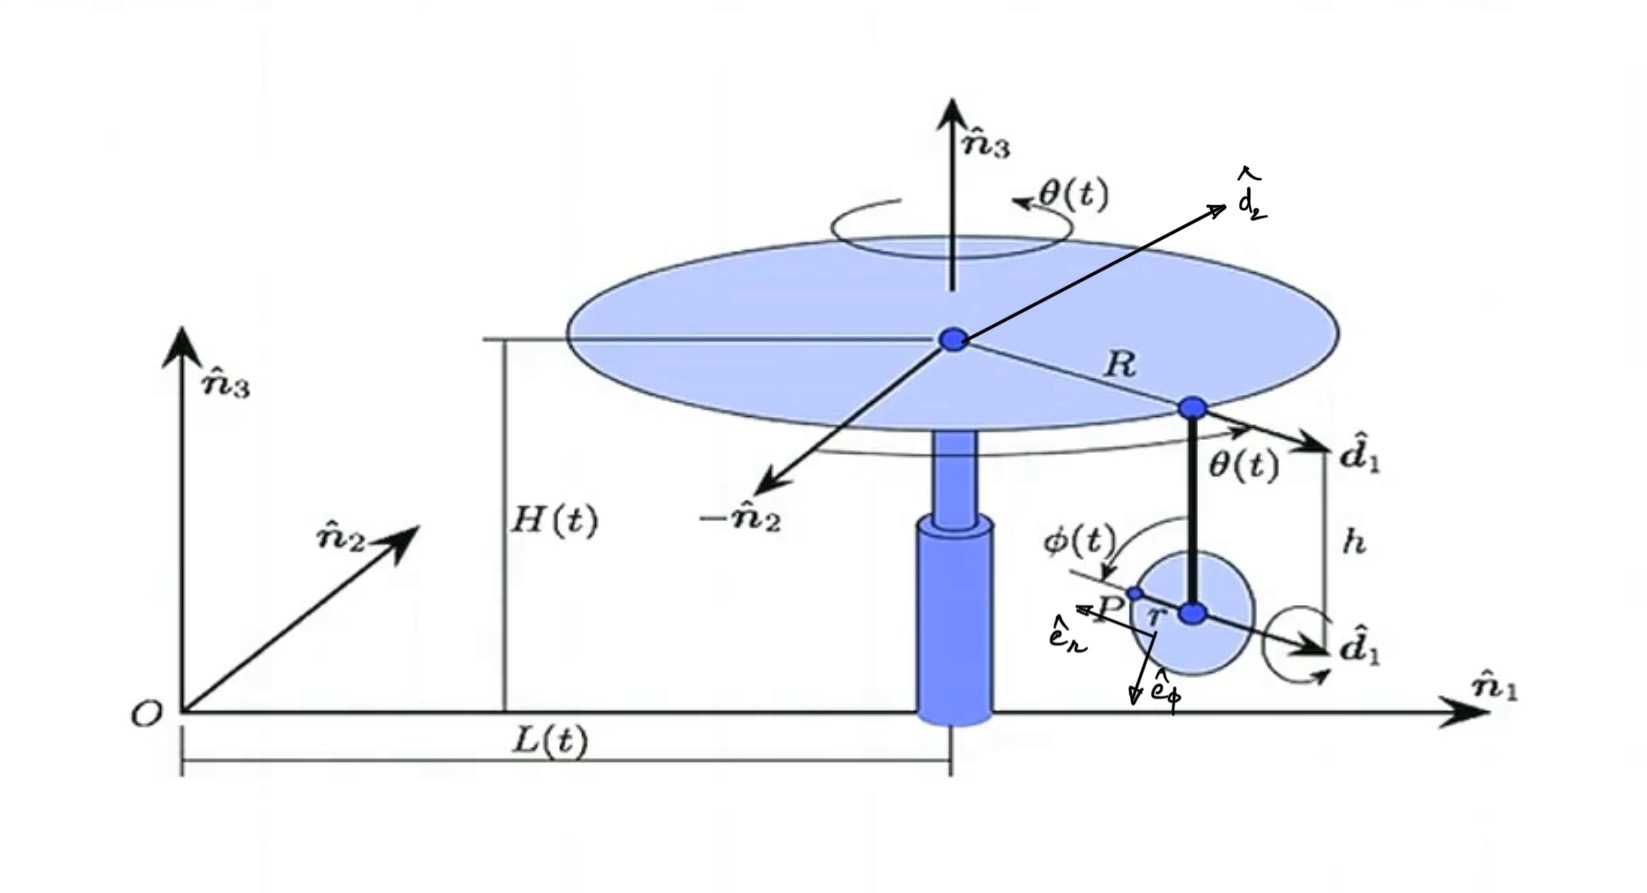
\includegraphics[width=\linewidth]{figures/dynamics/3D_transport_thm_ex.jpg}
		\caption{Figure for \autoref{ex:3dtransport_thm}}
		\label{fig:3dtansport_thm_ex}
	\end{figure}

	Assigning the frames we have,
	\[
		\begin{aligned}
			\mathcal{N} & \colon  \{ \bm{{\hat{n}_{1}}} , \bm{{\hat{n}_{2}}} , \bm{{\hat{n}_{3}}}  \}     \\
			\mathcal{D} & \colon  \{ \bm{{\hat{d}_{1}}} , \bm{{\hat{d}_{2}}} , \bm{{\hat{n}_{3}}}  \}     \\
			\mathcal{E} & \colon  \{ \bm{{\hat{e}_{r}}} , \bm{{\hat{e}_{\phi }}} , \bm{{\hat{d}_{1}}}  \} \\
		\end{aligned}
	\]
	And the angular velocities of the frames relative to each other can be expressed as:
	\[
		\begin{aligned}
			\bm{\omega _{\mathcal{D} / \mathcal{N} }} & = \dot{ \theta} \bm{{\hat{n}_{3}}}                                                    \\
			\bm{\omega _{\mathcal{E} / \mathcal{D} }} & = \dot{ \phi} \bm{{\hat{d}_{1}}}                                                      \\
			\bm{\omega _{\mathcal{E} / \mathcal{N} }} & = \bm{\omega _{\mathcal{D} / \mathcal{N} }}+\bm{\omega _{\mathcal{E} / \mathcal{D} }} \\
			                                          & = \dot{\theta } \bm{{\hat{n}_{3}}} + \dot{\phi } \bm{{\hat{d}_{1}}}                   \\
		\end{aligned}
	\]
	Thus,
	\[
		\begin{aligned}
			\bm{r}  & = L \bm{{\hat{n}_{1}}} + H \bm{{\hat{n}_{3}}} + R \bm{{\hat{d}_{1}}} - h \bm{{\hat{n}_{3}}}  + r \bm{{\hat{e}_{r}}} \\
			\dot{r} & = \prescript{\mathcal{N}}{}{\frac{d}{dt}}\bm{r}                                                                     \\
			        & = \dot{L} \bm{{\hat{n}_{1}}} + \dot{H} \bm{{\hat{n}_{3}}} +
			\left[ \cancelto{0}{
					\prescript{\mathcal{D}}{}{\frac{d}{dt}}R \bm{{\hat{d}_{1}}}
				} + \omega_{\mathcal{D} / \mathcal{N} } \times R \bm{{\hat{d}_{1}}}
				\right]
		\end{aligned}
	\]
\end{example}


    % Make the pagestyle fancy for the intro.tex page.
    \pagestyle{fancy}

    % Remove the line for the header.
    \renewcommand\headrulewidth{0pt}

    % Remove all header stuff.
    \fancyhead{}

    % Add stuff for the footer in the center.
    \fancyfoot[C]{
      \textit{For more notes like this, visit
      \href{\linktootherpages}{\shortlinkname}}. \\
      \vspace{0.1cm}
      \hrule
      \vspace{0.1cm}
      \@author, \\
      \term: \academicyear, \\
      Last Update: \@date, \\
      \faculty
    }
  }{ % If the intro.tex file doesn't exist.
    % Force a \newpageage.
    \forcenewpage
  }

  % Create a new page.
  \newpage

  % Remove the center stuff we did above, and replace it with just the page
  % number, which is still in roman numerals.
  \fancyfoot[C]{\thepage}
  % Add the table of contents.
  \tableofcontents
  % Force a new page.
  \forcenewpage

  % Move the page numberings back to arabic, from roman numerals.
  \pagenumbering{arabic}
  % Set the page number to 1.
  \setcounter{page}{1}

  % Add the header line back.
  \renewcommand\headrulewidth{0.4pt}
  % In the top right, add the lecture title.
  \fancyhead[R]{\nouppercase{\leftmark}}
  % In the top left, add the author name.
  % In the bottom center, add the page.
  \fancyfoot[C]{\thepage}
  % Add a nice gray background in the middle of all the upcoming pages.
  % \definegraybackground
}

\makeatother


%%%%%%%%%%%%%%%%%%%%%%%%%%%%%%%%%%%%%%%%%%%%%%%%%%%%%%%%%%%%%%%%%%%%%%%%%%%%%%%
%                               Custom Commands                               %
%%%%%%%%%%%%%%%%%%%%%%%%%%%%%%%%%%%%%%%%%%%%%%%%%%%%%%%%%%%%%%%%%%%%%%%%%%%%%%%

%%%%%%%%%%%%
%  Circle  %
%%%%%%%%%%%%

\newcommand*\circled[1]{\tikz[baseline=(char.base)]{
  \node[shape=circle,draw,inner sep=1pt] (char) {#1};}
}

%%%%%%%%%%%%%%%%%%%
%  Todo Commands  %
%%%%%%%%%%%%%%%%%%%

\usepackage{xargs}
\usepackage[colorinlistoftodos]{todonotes}

\makeatletter

\@ifclasswith\class{working}{
  \newcommandx\unsure[2][1=]{\todo[linecolor=red,backgroundcolor=red!25,bordercolor=red,#1]{#2}}
  \newcommandx\change[2][1=]{\todo[linecolor=blue,backgroundcolor=blue!25,bordercolor=blue,#1]{#2}}
  \newcommandx\info[2][1=]{\todo[linecolor=OliveGreen,backgroundcolor=OliveGreen!25,bordercolor=OliveGreen,#1]{#2}}
  \newcommandx\improvement[2][1=]{\todo[linecolor=Plum,backgroundcolor=Plum!25,bordercolor=Plum,#1]{#2}}

  \newcommand\listnotes{
    \newpage
    \listoftodos[Notes]
  }
}{
  \newcommandx\unsure[2][1=]{}
  \newcommandx\change[2][1=]{}
  \newcommandx\info[2][1=]{}
  \newcommandx\improvement[2][1=]{}

  \newcommand\listnotes{}
}

\makeatother

%%%%%%%%%%%%%
%  Correct  %
%%%%%%%%%%%%%

% EXAMPLE:
% 1. \correct{INCORRECT}{CORRECT}
% Parameters:
% 1. The incorrect statement.
% 2. The correct statement.
\definecolor{correct}{HTML}{009900}
\newcommand\correct[2]{{\color{red}{#1 }}\ensuremath{\to}{\color{correct}{ #2}}}


%%%%%%%%%%%%%%%%%%%%%%%%%%%%%%%%%%%%%%%%%%%%%%%%%%%%%%%%%%%%%%%%%%%%%%%%%%%%%%%
%                                 Environments                                %
%%%%%%%%%%%%%%%%%%%%%%%%%%%%%%%%%%%%%%%%%%%%%%%%%%%%%%%%%%%%%%%%%%%%%%%%%%%%%%%

\usepackage{varwidth}
\usepackage{thmtools}
\usepackage[most,many,breakable]{tcolorbox}

\tcbuselibrary{theorems,skins,hooks}
\usetikzlibrary{arrows,calc,shadows.blur}

%%%%%%%%%%%%%%%%%%%
%  Define Colors  %
%%%%%%%%%%%%%%%%%%%

\definecolor{myblue}{RGB}{45, 111, 177}
\definecolor{mygreen}{RGB}{56, 140, 70}
\definecolor{myred}{RGB}{199, 68, 64}
\definecolor{mypurple}{RGB}{197, 92, 212}

\definecolor{definition}{HTML}{7B0000}
\definecolor{theorem}{HTML}{00007B}
\definecolor{example}{HTML}{2A7F7F}
\definecolor{definition}{HTML}{228b22}
\definecolor{prop}{HTML}{191971}
\definecolor{lemma}{HTML}{983b0f}
\definecolor{exercise}{HTML}{88D6D1}

% \colorlet{definition}{mygreen!85!black}
\colorlet{claim}{mygreen!85!black}
\colorlet{corollary}{mypurple!85!black}
\colorlet{proof}{theorem}

%%%%%%%%%%%%%%%%%%%%%%%%%%%%%%%%%%%%%%%%%%%%%%%%%%%%%%%%%
%  Create Environments Styles Based on Given Parameter  %
%%%%%%%%%%%%%%%%%%%%%%%%%%%%%%%%%%%%%%%%%%%%%%%%%%%%%%%%%

\mdfsetup{skipabove=1em,skipbelow=0em}

%%%%%%%%%%%%%%%%%%%%%%
%  Helpful Commands  %
%%%%%%%%%%%%%%%%%%%%%%

% EXAMPLE:
% 1. \createnewtheoremstyle{thmdefinitionbox}{}{}
% 2. \createnewtheoremstyle{thmtheorembox}{}{}
% 3. \createnewtheoremstyle{thmproofbox}{qed=\qedsymbol}{
%       rightline=false, topline=false, bottomline=false
%    }
% Parameters:
% 1. Theorem name.
% 2. Any extra parameters to pass directly to declaretheoremstyle.
% 3. Any extra parameters to pass directly to mdframed.
\newcommand\createnewtheoremstyle[3]{
  \declaretheoremstyle[
  headfont=\bfseries\sffamily, bodyfont=\normalfont, #2,
  mdframed={
    #3,
  },
  ]{#1}
}

% EXAMPLE:
% 1. \createnewcoloredtheoremstyle{thmdefinitionbox}{definition}{}{}
% 2. \createnewcoloredtheoremstyle{thmexamplebox}{example}{}{
%       rightline=true, leftline=true, topline=true, bottomline=true
%     }
% 3. \createnewcoloredtheoremstyle{thmproofbox}{proof}{qed=\qedsymbol}{backgroundcolor=white}
% Parameters:
% 1. Theorem name.
% 2. Color of theorem.
% 3. Any extra parameters to pass directly to declaretheoremstyle.
% 4. Any extra parameters to pass directly to mdframed.
\newcommand\createnewcoloredtheoremstyle[4]{
  \declaretheoremstyle[
  headfont=\bfseries\sffamily\color{#2}, bodyfont=\normalfont, #3,
  mdframed={
    linewidth=2pt,
    rightline=false, leftline=true, topline=false, bottomline=false,
    linecolor=#2, backgroundcolor=#2!5, #4,
  },
  ]{#1}
}

%%%%%%%%%%%%%%%%%%%%%%%%%%%%%%%%%%%
%  Create the Environment Styles  %
%%%%%%%%%%%%%%%%%%%%%%%%%%%%%%%%%%%

\makeatletter
\@ifclasswith\class{nocolor}{
  % Environments without color.

  \createnewtheoremstyle{thmdefinitionbox}{}{}
  \createnewtheoremstyle{thmtheorembox}{}{}
  \createnewtheoremstyle{thmexamplebox}{}{}
  \createnewtheoremstyle{thmclaimbox}{}{}
  \createnewtheoremstyle{thmcorollarybox}{}{}
  \createnewtheoremstyle{thmpropbox}{}{}
  \createnewtheoremstyle{thmlemmabox}{}{}
  \createnewtheoremstyle{thmexercisebox}{}{}
  \createnewtheoremstyle{thmdefinitionbox}{}{}
  \createnewtheoremstyle{thmquestionbox}{}{}
  \createnewtheoremstyle{thmsolutionbox}{}{}

  \createnewtheoremstyle{thmproofbox}{qed=\qedsymbol}{}
  \createnewtheoremstyle{thmexplanationbox}{}{}
}{
  % Environments with color.

  \createnewcoloredtheoremstyle{thmdefinitionbox}{definition}{}{}
  \createnewcoloredtheoremstyle{thmtheorembox}{theorem}{}{}
  \createnewcoloredtheoremstyle{thmexamplebox}{example}{}{
    rightline=true, leftline=true, topline=true, bottomline=true
  }
  \createnewcoloredtheoremstyle{thmclaimbox}{claim}{}{}
  \createnewcoloredtheoremstyle{thmcorollarybox}{corollary}{}{}
  \createnewcoloredtheoremstyle{thmpropbox}{prop}{}{}
  \createnewcoloredtheoremstyle{thmlemmabox}{lemma}{}{}
  \createnewcoloredtheoremstyle{thmexercisebox}{exercise}{}{}

  \createnewcoloredtheoremstyle{thmproofbox}{proof}{qed=\qedsymbol}{backgroundcolor=white}
  \createnewcoloredtheoremstyle{thmexplanationbox}{example}{qed=\qedsymbol}{backgroundcolor=white}
}
\makeatother

%%%%%%%%%%%%%%%%%%%%%%%%%%%%%
%  Create the Environments  %
%%%%%%%%%%%%%%%%%%%%%%%%%%%%%

\declaretheorem[numberwithin=section, style=thmtheorembox,     name=Theorem]{theorem}
\declaretheorem[numbered=no,          style=thmexamplebox,     name=Example]{example}
\declaretheorem[numberwithin=section, style=thmclaimbox,       name=Claim]{claim}
\declaretheorem[numberwithin=section, style=thmcorollarybox,   name=Corollary]{corollary}
\declaretheorem[numberwithin=section, style=thmpropbox,        name=Proposition]{prop}
\declaretheorem[numberwithin=section, style=thmlemmabox,       name=Lemma]{lemma}
\declaretheorem[numberwithin=section, style=thmexercisebox,    name=Exercise]{exercise}
\declaretheorem[numbered=no,          style=thmproofbox,       name=Proof]{replacementproof}
\declaretheorem[numbered=no,          style=thmexplanationbox, name=Proof]{expl}
\declaretheorem[numberwithin=section, style=thmdefinitionbox,  name=Definition]{definition}



\makeatletter
\@ifclasswith\class{nocolor}{
  % Environments without color.

  \newtheorem*{note}{Note}

  \declaretheorem[numberwithin=section, style=thmquestionbox,   name=Question]{question}
  \declaretheorem[numberwithin=section, style=thmsolutionbox,   name=Solution]{solution}
}{
  % Environments with color.


  \newtcolorbox{note}[1][]{%
    enhanced jigsaw,
    colback=gray!20!white,%
    colframe=gray!80!black,
    size=small,
    boxrule=1pt,
    title=\textbf{Note:-},
    halign title=flush center,
    coltitle=black,
    breakable,
    drop shadow=black!50!white,
    attach boxed title to top left={xshift=1cm,yshift=-\tcboxedtitleheight/2,yshifttext=-\tcboxedtitleheight/2},
    minipage boxed title=1.5cm,
    boxed title style={%
      colback=white,
      size=fbox,
      boxrule=1pt,
      boxsep=2pt,
      underlay={%
        \coordinate (dotA) at ($(interior.west) + (-0.5pt,0)$);
        \coordinate (dotB) at ($(interior.east) + (0.5pt,0)$);
        \begin{scope}
          \clip (interior.north west) rectangle ([xshift=3ex]interior.east);
          \filldraw [white, blur shadow={shadow opacity=60, shadow yshift=-.75ex}, rounded corners=2pt] (interior.north west) rectangle (interior.south east);
        \end{scope}
        \begin{scope}[gray!80!black]
          \fill (dotA) circle (2pt);
          \fill (dotB) circle (2pt);
        \end{scope}
      },
    },
    #1,
  }

  \newtcbtheorem{Question}{Question}{enhanced,
    breakable,
    colback=white,
    colframe=myblue!80!black,
    attach boxed title to top left={yshift*=-\tcboxedtitleheight},
    fonttitle=\bfseries,
    title=\textbf{Question:-},
    boxed title size=title,
    boxed title style={%
      sharp corners,
      rounded corners=northwest,
      colback=tcbcolframe,
      boxrule=0pt,
    },
    underlay boxed title={%
      \path[fill=tcbcolframe] (title.south west)--(title.south east)
      to[out=0, in=180] ([xshift=5mm]title.east)--
      (title.center-|frame.east)
      [rounded corners=\kvtcb@arc] |-
      (frame.north) -| cycle;
    },
    #1
  }{def}

  \NewDocumentEnvironment{question}{O{}O{}}
  {\begin{Question}{#1}{#2}}{\end{Question}}

  \newtcolorbox{Solution}{enhanced,
    breakable,
    colback=white,
    colframe=mygreen!80!black,
    attach boxed title to top left={yshift*=-\tcboxedtitleheight},
    title=\textbf{Solution:-},
    boxed title size=title,
    boxed title style={%
      sharp corners,
      rounded corners=northwest,
      colback=tcbcolframe,
      boxrule=0pt,
    },
    underlay boxed title={%
      \path[fill=tcbcolframe] (title.south west)--(title.south east)
      to[out=0, in=180] ([xshift=5mm]title.east)--
      (title.center-|frame.east)
      [rounded corners=\kvtcb@arc] |-
      (frame.north) -| cycle;
    },
  }

  \NewDocumentEnvironment{solution}{O{}O{}}
  {\vspace{-10pt}\begin{Solution}{#1}{#2}}{\end{Solution}}
}
\makeatother

%%%%%%%%%%%%%%%%%%%%%%%%%%%%
%  Edit Proof Environment  %
%%%%%%%%%%%%%%%%%%%%%%%%%%%%

\renewenvironment{proof}[1][\proofname]{\vspace{-10pt}\begin{replacementproof}}{\end{replacementproof}}
\newenvironment{explanation}[1][\proofname]{\vspace{-10pt}\begin{expl}}{\end{expl}}

\theoremstyle{definition}

\newtheorem*{notation}{Notation}
\newtheorem*{previouslyseen}{As previously seen}
\newtheorem*{problem}{Problem}
\newtheorem*{observe}{Observe}
\newtheorem*{property}{Property}
\newtheorem*{intuition}{Intuition}

%%%%%%%%%%%%%%
% part on a seperate page
%%%%%%%%%%%%%%

\makeatletter
\renewcommand\part{%
%  \if@openright
%    \cleardoublepage
%  \else
    \clearpage
%  \fi
  \thispagestyle{plain}%
  \if@twocolumn
    \onecolumn
    \@tempswatrue
  \else
    \@tempswafalse
  \fi
  \null\vfil
  \secdef\@part\@spart}

\def\@part[#1]#2{%
    \ifnum \c@secnumdepth >-2\relax
      \refstepcounter{part}%
      \addcontentsline{toc}{part}{\thepart\hspace{1em}#1}%
    \else
      \addcontentsline{toc}{part}{#1}%
    \fi
    \markboth{}{}%
    {\centering
     \interlinepenalty \@M
     \normalfont
     \ifnum \c@secnumdepth >-2\relax
       \huge\bfseries \partname\nobreakspace\thepart
       \par
       \vskip 20\p@
     \fi
     \Huge \bfseries #2\par}%
    \@endpart}
    
\def\@spart#1{%
    {\centering
     \interlinepenalty \@M
     \normalfont
     \Huge \bfseries #1\par}%
    \@endpart}
\def\@endpart{\vfil\newpage}
\makeatother